\newpage
\section{Heap}
\begin{definition}[Heap binario]
	Un \textbf{albero} quasi completo.
\end{definition}
\begin{definition}[Albero binario completo]
	Un albero dove ogni nodo è foglia oppure ha due figli.
\end{definition}
\begin{definition}[Albero binario quasi completo]
	Se $h$ è l'altezza dell'albero, tutte le foglie hanno profondità $h$ oppure $h-1$. Tutti i nodi hanno $2$ figli eccetto al più $1$. Il nodo con un solo figlio, se esiste:
	\begin{itemize}
		\item ha profondità $h-1$
		\item tutti i nodi alla sua destra sono \textbf{foglie}
		\item e il suo unico figlio è un figlio \textbf{sinistro}
	\end{itemize}
\end{definition}

\begin{figure}[h]
	\begin{subfigure}{.5\textwidth}
		\centering
		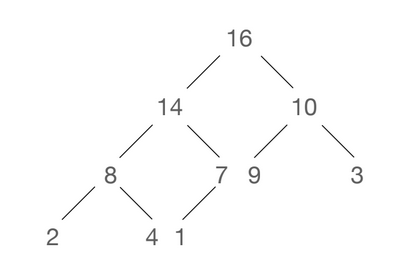
\includegraphics[width=6cm]{images/heap_tree.png}
		\caption{Albero binario quasi completo}
	\end{subfigure}
	\begin{subfigure}{.5\textwidth}
		\centering
		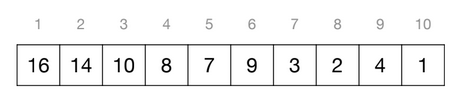
\includegraphics[width=6cm]{images/heap_array.png}
		\caption{Heap}
	\end{subfigure}
\end{figure}

\noindent
Di seguito alcune formule utili:
\begin{itemize}
	\item parent(i) = $\lfloor i/2 \rfloor$
	\item left(i) = $2i$
	\item right(i) = $2i+1$
\end{itemize}

\subsection{Max e min heap}
Dato un heap, se gli elementi di ogni sotto-albero sono più piccoli della radice del sotto-albero, allora abbiamo un \textbf{max-heap} e il massimo valore sarà memorizzato sempre nella radice.
\begin{equation}
	\forall i \neq 1, A[parent(i)] \geq A[i]
\end{equation}
Analogamente per il \textbf{min-heap} il minimo valore sarà nella radice.
\begin{equation}
	\forall i \neq 1, A[parent(i)] \leq A[i]
\end{equation}

\subsection{Proprietà}
\begin{itemize}
	\item \textbf{Proprietà 1}: un \textit{heap} di $n$ elementi ha altezza $\theta(\log{n})$, precisamente \color{red} $\lfloor \log{n} \rfloor$ \color{black}
	\item \textbf{Proprietà 2}: un \textit{heap} di $n$ elementi contiene \color{red} $\lceil n/2 \rceil$ \color{black} foglie
	\item \textbf{Proprietà 3}: un \textit{heap} di $n$ elementi ha al più \color{red} $\lceil n/2^{h+1} \rceil$ \color{black} nodi di altezza $h$, esattamente $\lceil n/2^{h+1} \rceil$ se è un albero \textit{bilanciato completo}
\end{itemize}